\documentclass[12pt,a4paper]{article}
\usepackage{graphicx}
\usepackage{geometry}
\usepackage{xcolor}
\usepackage{array}
\usepackage{longtable}
\usepackage{fancyhdr}
\usepackage{amsmath}
\geometry{margin=1in}
\usepackage{array}
\setlength{\headheight}{65pt}
\begin{document}
\noindent

\begin{center}
    \Large\textbf{\color{blue}Gate -2011-IN -16 Question}
\end{center}

\thispagestyle{fancy}
\fancyhf{}
\fancyhead[L]{
\includegraphics[height=1.5cm]{IIITB-COMET-Logo.png}}
\fancyhead[R]{
\begin{tabular}{r}
\textbf{Name:DARSI VAMSI} \\
\textbf{ID: COMETFWC071} \\
\end{tabular}
}
\section*{\color{blue}QUESTION}
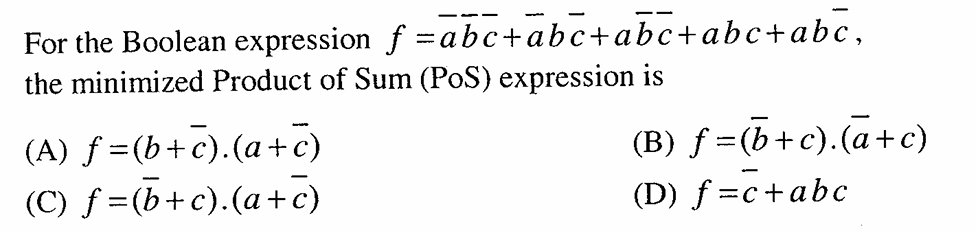
\includegraphics[width=1\textwidth,height=5 cm]{IN 2011 16-fpga.png}
\section*{\color{blue}QUESTION ANALYSIS}
\section*{Solution}

Assuming the Boolean expression is

$$
f=\bar{a}b\bar{c}+a\bar{b}\bar{c}+\bar{a}bc+abc+ab\bar{c}
$$

\subsection*{Step 1: Convert to Minterms}

$$
\bar{a}b\bar{c}=m_2
$$

$$
\bar{a}bc=m_3
$$

$$
a\bar{b}\bar{c}=m_4
$$

$$
ab\bar{c}=m_6
$$

$$
abc=m_7
$$

Therefore,

$$
f=\Sigma m(2,3,4,6,7)
$$

\subsection*{Step 2: Find the Zero Cells}

The missing minterms are

$$
m_0,\;m_1,\;m_5
$$

Hence,

$$
f=\Pi M(0,1,5)
$$

\subsection*{Step 3: K-map Grouping of Zeros}

\begin{center}
\begin{tabular}{|c|c|c|}
\hline
AB$\backslash$C & 0 & 1 \\
\hline
00 & 0 & 0 \\
\hline
01 & 1 & 1 \\
\hline
11 & 1 & 1 \\
\hline
10 & 1 & 0 \\
\hline
\end{tabular}
\end{center}

\paragraph{Group 1: $m_0$ and $m_1$}

Common variables:

$$
a=0,\qquad b=0
$$

Maxterm:

$$
(a+b)
$$

\paragraph{Group 2: $m_1$ and $m_5$}

Common variables:

$$
b=0,\qquad c=1
$$

Maxterm:

$$
(b+\bar{c})
$$

\subsection*{Step 4: Write the Minimized PoS Expression}

$$
\boxed{f=(a+b)(b+\bar{c})}
$$

\subsection*{Verification}

$$
(a+b)(b+\bar{c})
$$

is equal to 0 for

$$
000,\;001,\;101
$$

and equal to 1 for

$$
010,\;011,\;100,\;110,\;111
$$

which exactly matches the given function.

$$
\boxed{\text{Minimized PoS}=(a+b)(b+\bar{c})}
$$
\section*{Components Required}

\begin{center}
\begin{tabular}{|c|l|c|}
\hline
\textbf{S.No} & \textbf{Component} & \textbf{Quantity} \\
\hline
1 & Pygmy FPGA Board & 1 \\
\hline
2 & 7447 BCD-to-Seven-Segment Decoder IC & 1 \\
\hline
3 & Seven-Segment Display & 1 \\
\hline
4 & USB Cable & 1 \\
\hline
5 & Computer/Laptop (Linux/Ubuntu/Termux) & 1 \\
\hline
6 & FPGA Toolchain (QL SymbiFlow) & 1 \\
\hline
7 & Breadboard & 1 \\
\hline
8 & Connecting Wires & As Required \\
\hline

\end{tabular}
\end{center}
\section*{Hardware Connections}

\begin{center}
\begin{tabular}{|c|c|c|}
\hline
\textbf{Pygmy FPGA Pin} & \textbf{7447 IC Pin} & \textbf{Function} \\
\hline
15 & A & D0 (LSB) Input to 7447 \\
\hline
16 & B & D1 Input to 7447 \\
\hline
17 & C & D2 Input to 7447 \\
\hline
18 & D & D3 (MSB) Input to 7447 \\
\hline
11 & Input A & Boolean Function Input A \\
\hline
12 & Input B & Boolean Function Input B \\
\hline
13 & Input C & Boolean Function Input C \\
\hline
\end{tabular}
\end{center}

\vspace{0.5cm}

\begin{center}
\begin{tabular}{|c|c|c|}
\hline
\textbf{7447 IC Pin} & \textbf{Seven-Segment Display} & \textbf{Function} \\
\hline
a & Segment a & Top Segment \\
\hline
b & Segment b & Upper Right Segment \\
\hline
c & Segment c & Lower Right Segment \\
\hline
d & Segment d & Bottom Segment \\
\hline
e & Segment e & Lower Left Segment \\
\hline
f & Segment f & Upper Left Segment \\
\hline
g & Segment g & Middle Segment \\
\hline
COM & +5V & Common Anode Connection \\
\hline
\end{tabular}
\end{center}

\vspace{0.5cm}

\begin{center}
\begin{tabular}{|c|c|}
\hline
\textbf{Power Connections} & \textbf{Connection} \\
\hline
7447 VCC & +5V Supply \\
\hline
7447 GND & Ground \\
\hline
Seven-Segment COM & +5V \\
\hline
Pygmy GND & Common Ground with 7447 Circuit \\
\hline
\end{tabular}
\end{center}

\textbf{Note:}
\begin{itemize}
    \item Pygmy FPGA pins 11, 12, and 13 are used as inputs corresponding to variables \(A\), \(B\), and \(C\).
    \item The FPGA evaluates the Boolean function and generates a 4-bit BCD output on pins 15, 16, 17, and 18 (\(D_0\), \(D_1\), \(D_2\), and \(D_3\)).
    \item The 7447 IC decodes the BCD input and drives the seven-segment display.
    \item Since the 7447 is designed for common-anode displays, the COM pin of the display is connected to \(+5\,V\).
    \item All grounds must be connected together to establish a common reference.
\end{itemize}
\section*{Execution Procedure}

\begin{enumerate}

\item Create the Verilog source file \texttt{lcd_task.v} and the constraint file \texttt{lcd_task.pcf} in the working directory.

\item Compile the design using the QL SymbiFlow toolchain

\begin{verbatim}
ql_symbiflow -compile \
-d ql-eos-s3 \
-P pu64 \
-v lcd_task.v \
-t top \
-p lcd_task.pcf
\end{verbatim}

\item After successful compilation, the bitstream file is generated inside the \texttt{build} directory.

\begin{verbatim}
build/top.bit
\end{verbatim}

\item Rename the generated \texttt{.bit} file to a \texttt{.bin} file:

\begin{verbatim}
mv build/top.bit top.bin
\end{verbatim}

\item Copy the generated \texttt{.bin} file to the computer where the FPGA programming environment has been established.

\item Open a terminal and navigate to the directory containing the generated binary file:

\begin{verbatim}
cd <path_to_binary_file>
\end{verbatim}

\item Put the Pygmy FPGA board into Flash Mode and connect it to the computer using a USB cable.

\item Verify that the board is detected by the system:

\begin{verbatim}
ls -l /dev/ttyACM0
\end{verbatim}

If the device is detected, information about the serial port will be displayed.

\item Program the FPGA board using the TinyFPGA programmer utility:

\begin{verbatim}
python3 tinyfpga-programmer-gui.py \
--port /dev/ttyACM0 \
--m4app boolean_display_0.bin \
--node n4
\end{verbatim}

\item Wait until the programming process completes successfully.

\item Press the RESET button on the Pygmy FPGA board.

\item Observe the output on the hardware and verify the expected functionality.

\end{enumerate}
\section*{Results and Observations}

The designed Boolean function was successfully implemented on the Pygmy FPGA board and tested using a seven-segment display interfaced through the 7447 BCD-to-Seven-Segment Decoder IC. The FPGA received the input combinations through pins 11, 12, and 13 and generated the corresponding BCD output on pins 15, 16, 17, and 18. The 7447 decoder converted the BCD output into appropriate segment signals to display the digits \texttt{0} and \texttt{1}.

Figure~\ref{fig:hardware_output} shows the hardware setup and the output displayed on the seven-segment display during experimental verification.

\begin{figure}[h]
\centering
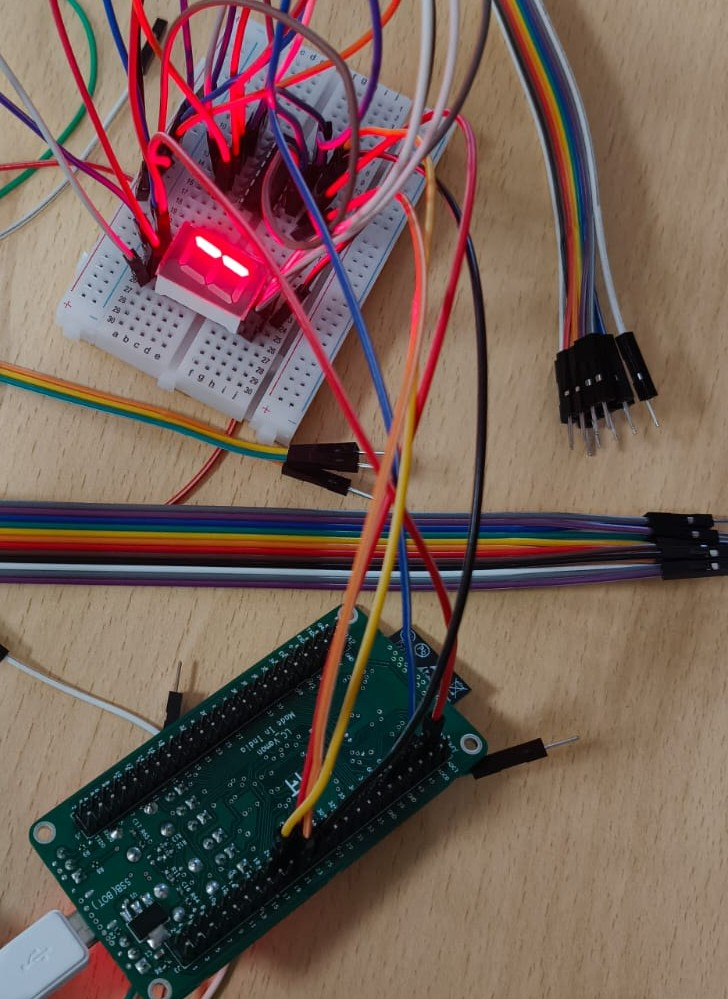
\includegraphics[width=0.55\textwidth]{7447_display_gate.jpeg}
\caption{Output Displayed on the Seven-Segment Display Using 7447 Decoder}
\label{fig:hardware_output}
\end{figure}

The output obtained from the hardware implementation was verified against the theoretical truth table. For each combination of inputs \(A\), \(B\), and \(C\), the displayed digit corresponded to the expected output of the Boolean function.

\subsection*{Observed Truth Table}

\begin{center}
\begin{tabular}{|c|c|c|c|}
\hline
\textbf{A} & \textbf{B} & \textbf{C} & \textbf{Displayed Digit} \\
\hline
0 & 0 & 0 & 0 \\
\hline
0 & 0 & 1 & 0 \\
\hline
0 & 1 & 0 & 1 \\
\hline
0 & 1 & 1 & 1 \\
\hline
1 & 0 & 0 & 1 \\
\hline
1 & 0 & 1 & 0 \\
\hline
1 & 1 & 0 & 1 \\
\hline
1 & 1 & 1 & 1 \\
\hline
\end{tabular}
\end{center}
\end{document}